\documentclass[4paper]{article}
\usepackage[spanish]{babel}
%\usepackage[ansinew]{inputenc}
\usepackage[utf8x]{inputenc}
%\usepackage[utf-8]{inputenc}
%\usepackage[T1]{fontenc}
\usepackage{graphicx}
\usepackage{multicol}
\usepackage{longtable}
\usepackage{array}
\usepackage{multirow}

\renewcommand{\tablename}{Tabla}

\author{Examen tercera evaluación}
\title{Tipo A}
\date{\today}

\begin{document}
\maketitle 
%\tableofcontents
%\newpage
\vspace{2cm}
\begin{center}
\begin{large}
%\textbf{Diagrama UML de la aplicación}
\end{large}
\end{center}\par 
%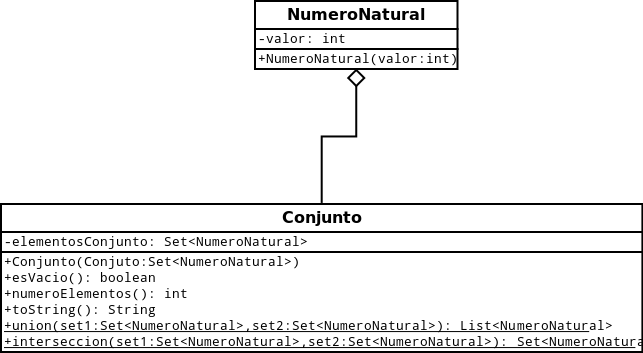
\includegraphics[scale=0.45]{UML.png}
\vspace{0.5cm}
\section*{Ejercicio 1}
Queremos realizar un programa para reservas turísticas, para esto debemos implementar como mínimo, las siguientes clases:
\begin{description}
\item[Reserva] que debe controlar el nombre, tiempo de instancia, es decir el número de noches, la fecha de reserva, número máximo de personas y si queremos media pensión, pension completa o no queremos pensión alguna. La fecha de reserva será la de creacción del objeto.
\item[ApartaHotel] donde controlamos el número de habitaciones y si la limpieza está incluida o no. En una habitación puede haber un máximo de dos personas.
\item[CasaRural] donde también controlamos el número de habitaciones, y si tiene piscina o no. En una habitación puede haber un máximo de dos personas.
\item[Hotel] donde debemos determinar si la habitación es doble o sencilla y el  número de estrellas de dicho hotel. En una habitación sencilla solo puede haber una persona y en la doble una o dos personas.
\end{description}
\begin{itemize}
\item Crea las correspondientes relaciones de herencia, puede añadir o quitar clases si lo ves conveniente, además es recomendable. Crea el correspondiente digrama UML.
\item Crea una excepción denominada \emph{NoInstanciaMinimaExcepcion} que se lance cuando se intente reservar con una instacia mínima inferior a dos noches. Comprueba su funcionamiento en el método main de la clase \emph{TestInstancia} y posteriormente déjala comentada (se comenta la creación de un objeto \emph{Estancia} que intente inicializarse con un tiempo de instancia inferior a dos noches).
\item Crea las siguientes reservas, objetos de tipo \emph{Estancia}, en el fichero \emph{TestInstancia}
\begin{itemize}
\item Estancia de 4 noches, para cinco personas, sin pensión de comida.
\item Estancia de 2 noches, para una persona y media pensión.
\item Estancia de 2 noches, para dos persona y pensión completa.
\end{itemize}
\item Los datos los obtienes leyéndolos del fichero agencia.csv (no tienes porque usar todos los campos). El tipo de pensión viene determinado por un número, 2 indica que incluye las tres opciones (completa, media o niguna), 1 que incluye dos opciones (media o ninguna) y 0 que no hay pensión alguna.
\item Para cada opción pude haber mas de un objeto \emph{Estancia} que satisfaga esas opciones, por lo que crea tres listas denominadas \emph{lista1, lista2 y lista3} y añadiras cada posibilidad a cada una de las listas. Es decir para el primer caso (estancia de 4 noches, para cinco personas, sin pensión de comida) a la primera lista, para el segundo caso (estancia de 2 noches, para una persona y media pensión) a la segunda lista y la otra lista para la última opción. En dichas listas debes añadir objetos de la clase \emph{Estancia}
\item En el caso de que el número de personas sea superior a dos, no contemples la opción de hotel.
\item Muestra por pantalla dichas posibilidades de reserva, es decir las tres listas antes creadas.
\item Vuelca estas tres colecciones en un fichero de texto, denominado \emph{outEstancia.txt}
\end{itemize}

\section*{Criterios de evaluacion}
Los criterios de evaluación son los indicados a continuación:\par 
\vspace*{0.5cm}
\begin{tabular}{|c|c|}
\hline
\textbf{CRITERIO EVALUACION} & \textbf{PUNTUACION} \\
\hline
Relaciones de herencia bien & 1 pto.\\
\hline
Fichero java de herencia bien & 2 ptos. \\
\hline
Excepción propia funcionando correctamente & 1 pto.\\
\hline
Lectura de los datos con Scanner & 2 ptos.\\
\hline 
Diagrama UML & 1 pto.\\
\hline
Lógica del archivo Test & 1.5 ptos.\\
\hline
Escritura de datos en archivo out.txt & 1.5 ptos.\\
\hline
\end{tabular}
\\
\\
En el caso de que no seas capaz de leer los datos para crear los objetos \emph{Estancia} del fichero \emph{estancias.csv} e incluirlos en las listas, puedes crearlo manualmente para posteriormente volcarlos al fichero \emph{out.txt} y pueda ser valorado. Lógicamente no se valorará la parte de lectura del fichero y parte de la lógica del fichero Test.
\section*{Subida de ficheros}
Comprime el directorio de trabajo de eclipse. Debes incluir el diagrama UML, bien en el propio directorio del proyecto o bien aparte. 
\end{document}
